\documentclass{book}
\usepackage[utf8]{vietnam}
\usepackage{cite}
\usepackage{amsmath,amssymb,amsfonts}
\usepackage{algorithm}
\usepackage{algorithmic}
\usepackage{graphicx}
\usepackage{textcomp}
\usepackage{xcolor}
\usepackage{tabularx}
\usepackage{listings}
\usepackage{enumerate}

\newcounter{savedenum}
\newcommand*{\saveenum}{\setcounter{savedenum}{\theenumi}}
\newcommand*{\resume}{\setcounter{enumi}{\thesavedenum}}


\begin{document}
%\title{TỐI ƯU LỒI VÀ ỨNG DỤNG TRONG HỌC MÁY HỌC}
%\author{Võ Thị Lưu Phương}
%
%
%\maketitle

\setcounter{chapter}{2}
\chapter{BÀI TOÁN TỐI ƯU LỒI}
\textit{Tác giả: Võ Thị Lưu Phương\\Email: vtlphuong@hcmiu.edu.vn}


\section{Giới thiệu bài toán tối ưu}
Một bài toán tối ưu có dạng chính tắc như sau:
\begin{align}
\mathrm{min.}~ & f_0(x) \label{eq:convexprob_obj}\\
\mathrm{s.t.}~ & f_i(x) \leq 0, i = 1, \ldots, m \label{eq:convexprob_ineqcon}\\
			& h_i(x) = 0, i = 1, \ldots, p, \label{eq:convexprob_eqcon}		
\end{align}
trong đó, 
$x \in \mathbb{R}^n$ là biến của bài toán tối ưu, 
$f_0$ là hàm mục tiêu, \eqref{eq:convexprob_ineqcon} và \eqref{eq:convexprob_eqcon} là các ràng buộc.

$p^*$ được gọi là \textit{nghiệm tối ưu} nếu $p^* = \min \{f_0(x) | f_i(x) \leq 0, i = 1,\ldots,m, h_i(x) = 0, i = 1, \ldots, p\}$.

Miền xác định của bài toán được định nghĩa là giao của các miền xác định của tất cả các hàm trong bài toán
\begin{align*}
\mathcal{D} = (\cap_{i=0}^m \rm{dom} f_i) \cap (\cap_{i=1}^p \rm{dom} h_i).
\end{align*}
Miền khả thi của bài toán được định nghĩa là tập hợp các điểm thỏa mãn các ràng buộc
\begin{align*}
\left\lbrace x  | x \in \mathcal{D}; f_i(x) \leq 0, i = 1, \ldots, m; h_i(x) = 0, i = 1, \ldots, p \right\rbrace
\end{align*}

Nếu bài toán không có chặn dưới thì $p^* = -\infty$ và nếu miền nghiệm là rỗng thì bài toán vô nghiệm ($p^* = \infty$).

$x^*$ được gọi là điểm cực tiểu (hay vector cực tiểu) nếu $x^*$ thuộc miền khả thi và $f_0(x^*) = p^*$.
Tập hợp tất các các điểm cực tiểu của bài toán thì được gọi là tập cực tiểu
\begin{align*}
X_{opt} = \{ x | x \in \mathcal{D} ~ \mathrm{and} ~ f_0(x) = p^*\}
\end{align*}

Một vector $x^*$ được gọi là vector cực tiểu cục bộ nếu tồn tại một số thực $R$ dương đủ nhỏ sao cho $f_0(x)$ đạt cực tiểu trong lân cận của $x^*$ bán kính $R$
\begin{align*}
f_0(x^*) = & \min \{f_0(z) | f_i(z)  \leq 0, i = 1, \ldots, m, \\
		& h_i(z) = 0, i = 1, \ldots, p, \|z - x^* \|_2 \leq R \},
\end{align*}

\section{Một số biến đổi bài toán tương đương}
Hai bài toán tối ưu được gọi là tương đương nếu ta có thể suy ra dễ dàng nghiệm của một bài toán nếu có nghiệm của bài toán kia.

Ví dụ có một số bài toán tối ưu mà ràng buộc dạng chận trên và chận dưới đơn giản như sau
\begin{align*}
\mathrm{min.}~ & f_0(x)\\
\mathrm{s.t.}~ & l_i \leq x_i \leq u_i, i = 1, \ldots, n.
\end{align*}
Ta có thể chuyển bài toán trên thành bài toán tối ưu dạng chính tắc như sau:
\begin{align*}
\mathrm{min.}~ & f_0(x)\\
\mathrm{s.t.}~ & l_i-  x_i \leq 0, i = 1, \ldots, n\\
			& x_i - u_i \leq 0, i = 1, \ldots, n.
\end{align*}

\subsection*{Bài toán tìm cực đại}
Đối với bài toán tìm cực đại
\begin{align*}
\mathrm{max.} ~ & f_0(x)\\
\mathrm{s.t.} ~ & f_i(x) \leq 0, i = 1, \ldots, m \\
			& h_i(x) = 0, i = 1, \ldots, p.
\end{align*}
ta có thể chuyển bài toán trên về thành tìm cực tiểu $- f_0(x)$.

\subsection*{Biến đổi các hàm mục tiêu và ràng buộc}
Một bài toán có hàm mục tiêu và các ràng buộc được nhân với các hằng số cũng là bài toán tương đương với bài toán gốc 
\begin{align*}
\mathrm{min.} ~ & \tilde{f}(x) = \alpha_0 f_0(x)\\
\mathrm{s.t} ~ & \tilde{f}_i (x) = \alpha_i f_i(x) \leq 0, i = 1, \ldots, m \\
			& \tilde{h}_i(x) = \beta_i h_i(x) = 0, i = 1, \ldots, p,
\end{align*}
trong đó $\alpha_i > 0, i=0, \ldots, m$ và $\beta_i \neq 0, i=1, \ldots, p$.

Ta cũng có thể đổi biến $x = \phi(z)$ để chuyển đổi bài toán tương đương miễn phép đổi biến $\phi$ là ánh xạ một - một:
\begin{align*}
\tilde{f}_i(z) = f_i(\phi(z)), i = 0, \ldots, m, \quad \tilde{h}_i(z) = h_i(\phi(z)), i = 0, \ldots, p.
\end{align*}
Do đó bài toán tương đương có được là:
\begin{align*}
\mathrm{min.}~ & \tilde{f}_0 (z) \\
\mathrm{st.}~ & \tilde{f}_i (z)  \leq 0, i = 1, \ldots, m \\
			& \tilde{h}_i(z) = 0, i = 1, \ldots, p
\end{align*}

Ta cũng có thể biến đổi tương đương các hàm mục tiêu và ràng buộc bằng các hàm riêng rẽ.
Cho $\psi_0: \mathbb{R}^n \rightarrow \mathbb{R}^n$ là hàm đơn điệu tăng,
$\psi_1, \ldots, \psi_m: \mathbb{R} \rightarrow \mathbb{R}$ thỏa mãn $\psi_i(u) \leq 0$ nếu và chỉ nếu $u \leq 0$, và 
$\xi_1, \ldots, \xi_{p}: \mathbb{R} \rightarrow \mathbb{R}$ thoả mãn $\xi_i(u) = 0$ nếu và chỉ nếu $u = 0$.
Định nghĩa các hàm số sau:
\begin{align*}
\tilde{f}_i(x) &= \psi_i(f_i(x)), i = 0, \ldots, m, \\
\tilde{h}_i(x) &= \xi_{i}(h_i(x)), i = 0, \ldots, p.
\end{align*}
Ta có bài toán sau tương được với bài toán gốc \eqref{eq:convexprob_obj}-\eqref{eq:convexprob_eqcon}
\begin{align*}
\mathrm{min.}~ & \tilde{f}_0 (x) \\
\mathrm{s.t.}~ & \tilde{f}_i (x)  \leq 0, i = 1, \ldots, m \\
			& \tilde{h}_i(x) = 0, i = 1, \ldots, p.
\end{align*}

Ví dụ các bài toán cực tiểu norm và cực tiểu norm bình phương là tương đương.
Thay vì giải bài toán gốc
\begin{align*}
\min ~ \| Ax - b \|_2.
\end{align*}
không khả vi tại một số điểm, ta có thể giải bài toán tương đương khả vi tại mọi điểm
\begin{align*}
\min ~ \| Ax - b \|_2^2 = (Ax - b)^T(Ax - b).
\end{align*}

\subsection*{Biến phụ}
Biến đổi bài toán tương đương có thể thực hiện bằng cách thêm vào \textit{biến phụ}.
Ví dụ bài toán sau tương được với bài toán gốc \eqref{eq:convexprob_obj}-\eqref{eq:convexprob_eqcon} bằng cách thêm biến $s_i, i = 1, \ldots, m$
\begin{align*}
\mathrm{min.}~ & f_0(x)\\
\mathrm{s.t.}~ & s_i \geq 0, i = 1, \ldots, m \\
			& f_i(x) + s_i = 0, i = 1, \ldots, m \\
			& h_i(x) = 0, i = 1, \ldots, p.
\end{align*}

\subsection*{Lược bớt và thêm ràng buộc đẳng thức}
Ta cũng có thể lược bớt ràng buộc đẳng thức nếu có hàm số $\phi$ sao cho $h_i(x) = 0,  i = 1, \ldots, p$ nếu và chỉ nếu $x = \phi(z)$, thì ta có bài toán sau tương đương với bài toán gốc \eqref{eq:convexprob_obj}-\eqref{eq:convexprob_eqcon}.
\begin{align*}
\mathrm{minimization}~ & \tilde{f}(z) = f_0(\phi(z)) \\
\mathrm{subject ~ to}~ & \tilde{f}_i (z)  = f_i(\phi(z)) \leq 0, i = 1, \ldots, m.
\end{align*}

Thêm ràng buộc đẳng thức
Hai bài toán sau là tương đương:
\begin{align*}
\mathrm{min.}~ & f_0(A_0 x + b_0)\\
\mathrm{s.t.}~ & f_i(A_i x + b_i) \leq 0, i = 1, \ldots, m \\
			& h_i(x) = 0, i = 1, \ldots, p.
\end{align*}
và
\begin{align*}
\mathrm{min.}~ & f_0(y_0)\\
\mathrm{s.t.}~ & f_i(y_i) \leq 0, i = 1, \ldots, m \\
			& y_i = A_i x + b_i, i = 0, \ldots, m \\
			& h_i(x) = 0, i = 1, \ldots, p.
\end{align*}

\subsection*{Tối ưu trên một vài biến}
Ta cũng có thể thực hiện \textit{tối ưu trên một vài biến} đối với một số bài toán dạng đăc biệt. Ví dụ như bài toán có hai nhóm ràng buộc độc lập giữa $x_1$ và $x_2$ sau
\begin{align*}
\mathrm{min.}~ & f_0(x_1, x_2)\\
\mathrm{s.t.}~ & f_i(x_1) \leq 0, i = 1, \ldots, m_1\\
				& g_i(x_2) \leq 0, i = 1, \ldots, m_2
\end{align*}
sẽ tương đương với bài toán
\begin{align*}
\mathrm{min.}~ & \tilde{f}_0(x_1)\\
\mathrm{s.t.}~ & f_i(x_1) \leq 0, i = 1, \ldots, m_1,
\end{align*}
trong đó
\begin{align*}
\tilde{f}_0(x_1) = \min_{x_2 | g_i(x_2) \leq 0, i = 1,...,m_2} f_0(x_1, x_2).
\end{align*}


\subsection*{Biến đổi dạng epigraph}
Bài toán dạng epigraph sau là tương đương với bài toán gốc
\begin{align*}
\mathrm{min.}~ & t\\
\mathrm{s.t.}~ & f_0(x) - t \leq 0 \\
			& f_i(y_i) \leq 0,  \quad i = 1, \ldots, m \\
			& h_i(x) = 0, 		\quad i = 1, \ldots, p.
\end{align*}
$(x^*, t^*)$ là cực tiểu của bài toán dạng epigraph nếu và chỉ nếu $x^*$ là điểm cực tiểu của bài toán gốc và đồng thời $t^* = f_0(x^*)$.

\section{Bài toán tối ưu lồi}

Bài toán tối ưu lồi có dạng như sau
\begin{align*}
\mathrm{min.}~ & f_0(x)\\
\mathrm{s.t.}~ & f_i(x) \leq 0, \quad i = 1, \ldots, m \\
			& a_i^T x = b_i, 	\quad i = 1, \ldots, p.
\end{align*}
Trong đó, các hàm mục tiêu và ràng buộc bất đăng thức $f_i, i=1, \ldots, m$ đều là hàm lồi. 
Ràng buộc dạng đẳng thức phải ở dạng tuyến tính.

Từ tính chất giao các tập lồi là tập lồi và epigraph của một hàm lồi là một tập lồi, ta có miền khả thi của một bài toán tối ưu lồi là một tập lồi.

\subsection{Bài toán tìm cực đại hàm lõm}
Bài toán tìm cực đại 
\begin{align}
\mathrm{max.}~ & f_0(x) \label{eq:convprob_obj}\\
\mathrm{s.t.}~ & f_i(x) \leq 0, \quad i = 1, \ldots, m \label{eq:convprob_incon}\\
			& a_i^T x = b_i, 	\quad i = 1, \ldots, p, \label{eq:convprob_affcon}
\end{align}
trong đó trong đó $f_0$ là hàm lõm và các hàm $f_i, i=1,...,m$ lồi cũng được xem là bài toán tối ưu lồi.

\subsection{Điểm cực trị}
Trong bài toán tối ưu lồi, điểm cực trị cục bộ cũng là điểm cực trị toàn cục.
%Vui lòng xem chứng minh ờ trang 138 sách \cite{boyd}.

Giả sử \emph{miền khả thi} của bài toán là là $X = \{ x | f_i(x) \leq 0, i=1, \ldots, m, h_i(x) = 0, i = 1, \ldots, p \}$. Trong trường hợp hàm $f_0$ khả vi,
$x^*$ là điểm cực trị nếu và chỉ nếu $x^* \in X$ và 
\begin{align*}
\nabla f_0(x^*)^T (y - x^*) \geq 0, \quad \forall y \in X.
\end{align*}


Đặc biệt nếu bài toán tối ưu không có ràng buộc thì điều kiện cần và đủ để $x^*$ cực trị là
\begin{align*}
\nabla f_0(x) = 0
\end{align*}
Ví dụ trong bài toán tối ưu một hàm toàn phương 
\begin{align*}
\min f_0(x) = (1/2) x^T Px + q^T x + r,
\end{align*}
trong đó ma trận $P$ đối xứng và xác định dương, điều kiện cần và đủ để $x^*$ cực trị  là $Px^* + q = 0$.
Từ đó, ta có nghiệm của bài toán là $x^* = -P^{-1}q$ nếu ma trận $P$ xác định dương chặt. 
Nếu $det(P) = 0$ ($P$ singular) thì $x^* = -P^{\dagger} q + \mathcal{N} (P)$, trong đó  $P^\dagger = (P^T P)^{-1} P^T$.

\subsection{Một số ví dụ về bài toán tối ưu lồi}
\subsubsection*{Linear programming}
Bài toán quy hoạch tuyến tính là một bài toán tối ưu lồi.
\begin{align*}
\mathrm{min.}~ & c^T x + d \\
\mathrm{s.t.}~ & Gx \preceq h \\
			& A x = b,
\end{align*}
trong đó $G \in \mathbb{R}^{m \times n}$ và  $A \in \mathbb{R}^{p \times n}$.

Các biến đổi tương đương sau vẫn bảo toàn tính lồi bến bài toán gốc là lồi.
\begin{itemize}
\item Dạng epigraph của một bài toán lồi cũng là một bài toán lồi.
\item Thêm biến phụ $s_i$ tương ứng với ràng buộc $f_i(x) \leq 0$ để biến ràng buộc này thành ràng buộc dạng đẳng thức.
\item Bài toán tối ưu trên một số biến trong trường hợp bài toán gốc có các ràng buộc độc lập theo các biến vẫn là bài toán lồi (xem phần 3.2).
\end{itemize}


\subsubsection*{Bài toán tối ưu hàm toàn phương}
Bài toán tối ưu hàm toàn phương có dạng sau
\begin{align*}
\mathrm{min.}~ & (1/2) x^T P x + q^T x + r \\
\mathrm{s.t.}~ & Gx \leq h \\
			& A x = b,
\end{align*}
trong đó $P \in \mathbb{R}^{n \times n}, P \succeq 0$, $G \in \mathbb{R}^{m \times n}$ và  $A \in \mathbb{R}^{p \times n}$.
Bài toán trên là một bài toán tối ưu lồi.

Bài toán tối ưu trong \textit{hồi quy tuyến tính} (linear regression hay còn gọi là least square) chính là một bài toán tối ưu hàm toàn phương 
\begin{align*}
\| Ax - b\|^2_2 = x^T A^T A x - 2b^T A x + b^T b.
\end{align*}
Nghiệm của bài toán tối ưu trên là $x^* = A^\dagger b$, trong đó $A^\dagger = (A^T A)^{-1} A^T$ là ma trận nghịch đảo giả (Moore-Penrose pseudo-inverse) của ma trận A, được xem là dạng tổng quát của phép nghị đảo ma trận trong trường hợp ma trận không vuông hay không khả nghịch.
Một số bài toán hồi quy tuyến tích còn có thêm chận trên và chận dưới cho các biến, ví dụ, $l \preceq x \preceq u$.

%\textcolor{red}{Distance between polyhedra}:
%Define $\mathbf{dist}(\mathcal{P}_1, \mathcal{P}_2) =\min \| x_1 - x_2\|_2$, $x_1 \in \mathcal{P}_1, x_1 \in \mathcal{P}_2$. The problem is as follows:
%\begin{align*}
%\min ~& \| x_1 - x_2\|_2^2 \\
%\mathrm{s.t.} ~& A_1 x_1 \preceq b_1, \quad A_2 x_2 \preceq b_2.
%\end{align*}

%Bài toán tối ưu porfolio trong tài chính cũng có thể mô hình dưới dạng một bài toán tối ưu hàm toàn phương
%\begin{align*}
%\mathrm{min.}~ & \bar{c}^T x + \gamma x^T \Sigma x = \mathbb{E} c^T x + \gamma \mathbf{var}(c^T x) \\
%\mathrm{s.t.}~ & Gx \preceq h \\
%			& A x = b.
%\end{align*}
%Trong đó,
%\begin{itemize}
%\item Vector chi phí $c \in \mathbb{R}^n$ có giá trị ngẫu nhiên với mean là $\hat{c}$ và covariance $\Sigma = \mathbb{E}(c - \bar{c})(c - \bar{c})^T$.
%\item Given $x$, $c^T x$ is a random variable with mean $\mathbb{E} c^T x =  \bar{c}^T x$ and variance $x^T \Sigma x$
%\item $\gamma >0$ là tham số về rủi ro, thể hiện quan hệ tỷ lệ nghịch giữa chi phí và variance (mức độ rủi ro) 
%\end{itemize}

\subsubsection*{Geometric programming}
Bài toán tối ưu geometric programming xuất hiện trong một số lĩnh vực trong kỹ thuật, kinh tế, khoa học quản lý,... Ta có thể đưa bài toán geometric programming thành bài toán lồi tương đương.

Ta  có một số định nghĩa trước khi định nghĩa bài toán geometric programming như sau:
Hàm đơn thức (monomial) được định nghĩa là $f(x) = c x_1^{a_1} x_2^{a_2} \ldots x_n^{a_n}$, trong đó $c > 0, a_i \in \mathbb{R}$.
Hàm đa thức (posynomial) là hàm có dạng như sau $f(x) = \sum_{k = 1}^K c x_1^{a_{1k}} x_2^{a_{2k}} \ldots x_n^{a_{nk}}$, $c_k > 0$.

Bài toán tối ưu có dạng 
\begin{align*}
\mathrm{min.}~ & f_0(x)\\
\mathrm{s.t.}~ & f_i(x) \leq 1, \quad i = 1, \ldots, m \\
			& h_i(x) = 1, 	\quad i = 1, \ldots, p,
\end{align*}
trong đó $f_0, \ldots, f_m$ đều là posynomial, $h_i$ là monomial được gọi là bài toán tối ưu dạng \emph{geometric programming}.

Bằng cách thay biến $y_i = \log x_i$ và lấy logarit các hàm, ta có
\begin{itemize}
\item đơn thức $f(x) = c x_1^{a_1} x_2^{a_2} \ldots x_n^{a_n}$ trở thành
\begin{align*}
\log f(e^{y_1}, \ldots, e^{y_n})= a^T y + b
\end{align*}
trong đó $b = \log c$,
\item posynomial  $f(x) = \sum_{k = 1}^K c x_1^{a_{1k}} x_2^{a_{2k}} \ldots x_n^{a_{nk}}$ trở thành
\begin{align*}
\log f(e^{y_1}, \ldots, e^{y_n})= \log\Big(\sum_{i=1}^K e^{a_{ik}^T + b_{ik}}\Big),
\end{align*}
trong đó $b_k = \log c_k$,
\end{itemize}

Do đó, geometric program tương đương với bài toán tối ưu lồi sau
\begin{align*}
\mathrm{max.}~ & \log\Big(\sum_{i=1}^K e^{a_{0k}^T + b_{0k}}\Big)\\
\mathrm{s.t.}~ & \log\Big(\sum_{i=1}^K e^{a_{ik}^T + b_{ik}}\Big) \leq 1, \quad i = 1, \ldots, m \\
			& Gy + d = 0, 	\quad i = 1, \ldots, p.
\end{align*}

\section{MỘT SỐ BÀI TOÁN TỐI ƯU TRONG HỌC MÁY}
\subsection{Hồi quy tuyến tính}
Giả sử số ca mắc sốt xuất huyết và lượng mưa trong tháng qua thống kê trong 3 năm được mô tả ở Hình \ref{fig:linear_regression_scatter}, trong đó
\begin{align*}
x_1 =& [55,	102,	169,	177,	185,	236,	252,	269,	359,	380,	386,	115,\\
& 11,	 16,	137,	149,	216,	234,	251,	253,	356,	364,	372,	362,\\
& 36,	58,	63,	77,	282,	287,	304,	305,	370,	374,	399,	279]\\
y =&[163,	239,	227,	364,	265,	354,	325,	364,	577,	529,	544,	214\\
& 109,	9,	155,	179,	339,	434,	410,	373,	546,	486,	536,	471,\\
& 189,	275,	51,	184,	293,	501,	431,	462,	457,	514,	486,	461]
\end{align*}
%\noindent\begin{tabular}{|c|p{1.5cm}|p{1.5cm}||p{1.5cm}|p{1.5cm}||p{1.5cm}|p{1.5cm}|}
%\hline
%Tháng & Lượng mưa (mm) ($x_{i1}$)	&	Số ca/ 1 triệu dân ($y_i$)&Lượng mưa (mm) ($x_{i1}$)	&	Số ca/ 1 triệu dân ($y_i$)&Lượng mưa (mm) ($x_{i1}$)	&	Số ca/ 1 triệu dân ($y_i$)\\
%\hline
%1	& 14	& 51	& 15	& 30	& 16	& 49\\
%2	& 4		& 14	& 8		& 26	& 5		& 17\\
%3	& 9		& 27	& 11	& 21	& 11	& 31\\
%4	& 51	& 160	& 51	& 161	& 53	& 58\\
%5	& 213	& 428	& 213	& 643	& 216	& 650\\
%6	& 309	& 618	& 313	& 313	& 309	& 928\\
%7	& 295	& 299	& 296	& 889	& 295	& 595\\
%8	& 271	& 547	& 272	& 274	&272	& 545\\
%9	& 342	& 693	&345	& 699	& 344	& 693\\
%10	& 260	& 264	& 263	& 792	& 262	& 271\\
%11	& 119	& 242	& 124	& 255	& 122	& 373\\
%12	& 47	& 100	& 52	& 157	& 49	& 157\\
%\hline
%\end{tabular}
\par \textit{Ghi chú: Số liệu trên chỉ cho ví dụ minh họa này.}

\begin{figure}[h]
	\centering
	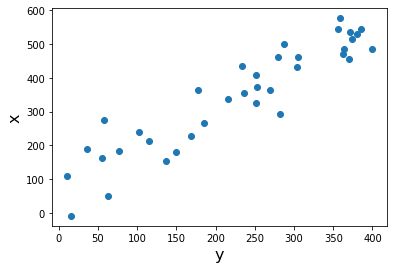
\includegraphics[width=7cm]{hinh_chuong3_convexprob/xy_plot.png}
	\caption{Tập dữ liệu ví dụ minh họa linear regression.}
	\label{fig:linear_regression_scatter}	
\end{figure}

\emph{Tìm hàm tuyến tính xấp xỉ số ca mắc ($y$) theo lượng mưa ($X$)}.

Giả sử một mẫu thứ $i$ có lương mưa là $x_{i1}$. 
Nếu ta thêm $x_0$ luôn bằng 1. Số ca mắc dự đoán tương ứng với lượng mưa sẽ được cho bởi hàm $f(w; x) = w_0 + x_{i1} w_1 = x^Tw$, trong đó, $x = [x_0, x_1]^T$. Trong khi đó giá thực là $y_i$.
Do đó sai số của ước lượng so với số ca thực của tập dữ liệu thường được lượng hóa bởi hàm norm:
\begin{align*}
L = ||y - Xw||,
\end{align*}
trong đó, 
$X = \begin{bmatrix} x_1^T \\ ... \\ x_{36}^T
\end{bmatrix}$, $y = \begin{bmatrix} y_1 \\ ... \\ y_{36}
\end{bmatrix}$

Ta cần tìm $w = [w_0, w_1]^T$ sao cho hàm ước lượng là khớp nhất với tập dữ liệu đã cho.
Điều đó có nghĩa là tổng sai số 
\begin{align*}
L = ||y - Xw||
\end{align*}
phải là nhỏ nhất.

Như vậy bài toán hồi quy tuyến tính được đưa về bài toán tối ưu lồi với biến $w$:
\begin{align*}
\mathrm{min.} ~ L = ||y - Xw||.
\end{align*}

Nếu dùng $\ell_2$-norm ước lượng khoảng cách giữa giá trị ước lượng và giá trị thật, ta thường tối thiểu hàm $\ell_2$-norm bình phương (có tên thông dụng là least square):
\begin{align*}
\mathrm{min.} ~ \frac{1}{2}||y - Xw||_2^2 = (y - Xw)^T (y - Xw).
\end{align*}

Dùng thư viện CVX, ta có thể tìm được vector trọng số $w=[77.80,  1.18]$.
\begin{figure}[h]
	\centering
	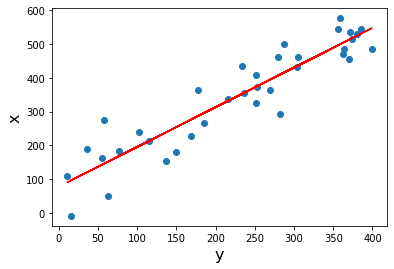
\includegraphics[width=7cm]{hinh_chuong3_convexprob/xy_plot_linear-regression.png}
	\caption{Hàm tuyến tính nội suy từ lượng mưa ra số ca mắc sốt xuất huyết.}
	\label{fig:convexset}	
\end{figure} 
%\subsection{Giải bài toán quy hoạch tuyến tính dùng CVXPY}

Nếu tập dữ liệu lớn với nhiều mẫu và nhiều đặc tính, bài toán tối ưu trở thành một bài toán kích thước lớn. Khi đó ta thường dùng giải thuật như gradient, stochastic gradient để giải bài toán.

Dùng hàm mất mát là $\ell_2$-norm thường khá nhạy cảm với các điểm đăc biệt. Ví dụ tập dữ liệu có điểm đặc biệt như Hình \ref{fig:linear_regression_outlier}. Nếu sử dụng hàm mất mát là $\ell_1$-norm sẽ cho kết quả trông tốt hơn như Hình \ref{fig:ell2_vs_ell1}.
\begin{figure}[h]
	\centering
	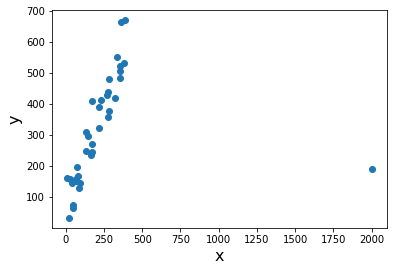
\includegraphics[width=7cm]{hinh_chuong3_convexprob/xy_plot_outlier.png}
	\caption{Tập dữ liệu với điểm đăc biệt.}
	\label{fig:linear_regression_outlier}	
\end{figure}

\begin{figure}[h]
	\centering
	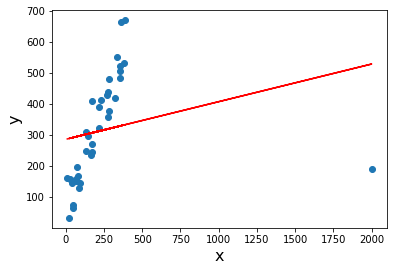
\includegraphics[width=6cm]{hinh_chuong3_convexprob/xy_linear-regression_outlier_ell2.png}
	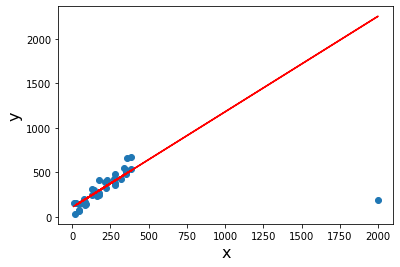
\includegraphics[width=6cm]{hinh_chuong3_convexprob/xy_linear-regression_outlier_ell1.png}
	\caption{Tối ưu với hàm mất mát là $\ell_2$-norm (trái) và $\ell_1$-norm (phải).}
	\label{fig:ell2_vs_ell1}	
\end{figure}

%\subsection{Fitting với các basic khác nhau}

\subsection{Bài toán logistic regression}
Trong các giải thuật phân lớp, đầu vào vector đăc tính $x$, đầu ra phải phân vào một trong $K$ lớp. 
Có hai phương pháp phổ biến trong phân lớp: 1) ước lượng hàm phân lớp trực tiếp từ tập dữ liệu cho trước, từ đó xác định $x$ thuộc lớp nào từ hàm này và 2) từ tập dữ liệu cho trước, tìm mô hình xác suất để ước lượng xác suất đối tượng với vector đặc tính $x$.
Trong phần này, chúng ta xem xét phương pháp thứ hai.

%\subsection{Bài toán fitting và maximum likelihood} 
%Trước tiên ta tìm hiểu khái niệm maximum likelihood.

Xét bài toán phân 2 lớp $C_1, C_2$ trong ví dụ sau:

Ta dùng hàm sigmoid để mô hình xác suất của đối tượng có vector đặc tính $x$ thuộc lớp $C_1$
\begin{align*}
p(C_1 | x) = \sigma(w^T x) = \frac{1}{1 + e^{-w^Tx}}.
\end{align*}
Như vậy $p(C_2 | x) = 1- p(C_1 | x)$ sẽ là xác suất đối tượng có vector đặc tính $x$ thuộc lớp $C_2$.
\begin{figure}[h]
	\centering
	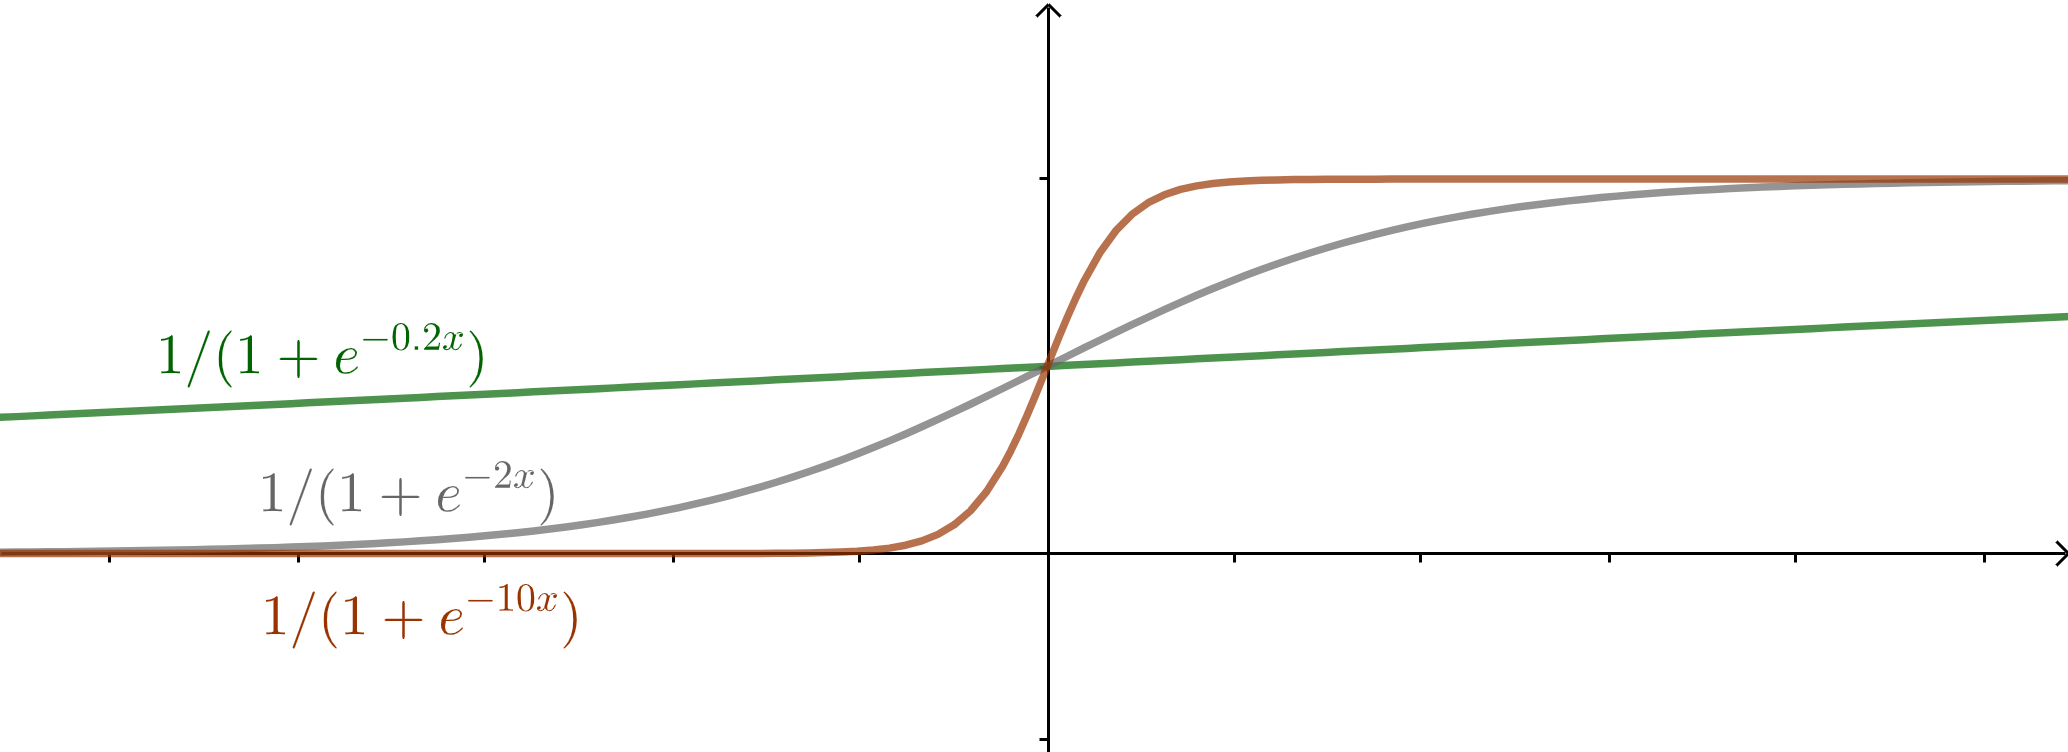
\includegraphics[width=9.5cm]{hinh_chuong2_convexfunc/chap2_sigmoid.png}
	\caption{Biểu diễn hàm sigmoid $\frac{1}{1 + e^{-w^Ta}}$ với $w = 0,2; 2; 10$ trong không gian 2D.}
	\label{fig:sigmoid}	
\end{figure}

Ta có một số tính chất của hàm sigmoid:
\begin{itemize}
\item Hàm sigmoid luôn có giá trị từ 0 đến 1, nên rất phù hợp để mô hình xác suất,
\item $\sigma(-a) = 1-\sigma(a)$.
\item Hàm nghịch đảo của hàm sigmoid được gọi là hàm \emph{logit}, 
\begin{align*}
a=\log(\frac{\sigma}{1-\sigma}) 
\end{align*}
\item Đạo hàm 
\begin{align*}
\frac{d \sigma}{da} = \sigma (1- \sigma).
\end{align*}
\end{itemize}

Cho dataset $(X, y)$, trong đó, $X = \begin{bmatrix} x_1^T \\ ... \\ x_N^T \end{bmatrix}$ là ma trận chứa $N$ vector đăc tính, $y = \begin{bmatrix} y_1^T \\ ... \\ y_N \end{bmatrix}$, $y_i$ là 0 hoặc 1. Vector $y$ còn được gọi là target. 
Ta tìm vector $w$ sao cho likelihood của tập dữ liệu theo mô hình xác suất $ \sigma(w^T x)$ là cực đại.

Do $y_i$ bằng 0 hoặc 1 trong bài toán phân hai lớp, ta có thể viết lại xác suất ước lượng theo mô hình sigmoid (likelihood) của vector $x_i$ theo dạng sau:
\begin{align}
P(y_i | x_i;w) = \sigma(w^T x_i)^{y_i} (1-\sigma(w^T x_i))^{1-y_i}.
\end{align} 
Theo công thức trên, nếu $y_i = 1$ (thuộc lớp $C_1$) thì xác xuất sẽ là $\sigma(w^T x_i)$ và nếu $y_i = 0$ (thuộc lớp $C_2$) thì xác xuất sẽ là $1-\sigma(w^T x_i)$.

Do đó, xác suất ước lượng theo sigmoid cho cả tập dữ liệu là
\begin{align}
P(y | X ;w) = \prod_{i=1}^N \sigma(w^T x_i)^{y_i} (1-\sigma(w^T x_i))^{1-y_i}.
\label{eq:likelihood}
\end{align} 

Ta cần tìm vector trọng số $w$ để tối đa xác suất ước lượng $P(y | X ;w)$ (maximum likelihood estimation).
Tuy nhiên thay vì tìm cực đại hàm số $P(y | X ;w)$ có dạng tích khá phức tạp, ta lấy logarit để biến đổi từ dạng tích về dạng tổng và tìm cực trị của hàm mục tiêu mới:
\begin{align*}
\log(P(y | X ;w)) &= \sum_{i=1}^N y_i \log(\sigma(w^T x_i)) + (1-y_i)\log (1-\sigma(w^T x_i))\\
				& = \sum_{i=1}^N y_i w^T x_i + \log (1-\sigma(w^T x_i)) \\
				& = \sum_{i=1}^N y_i w^T x_i - \log (1 + e^{w^T x_i}).
\end{align*}

Do đó bài toán được đưa về bài toán tìm cực trị của hàm log-likelihood:
\begin{align}
\mathrm{max.} \sum_{i=1}^N y_i w^T x_i - \log (1 + e^{w^T x_i}).
\end{align}


\subsection{Bài toán phân $K$ lớp với hàm softmax}

Nếu có nhiều hơn 2 lớp, ngõ ra $y$ được biểu diễn dưới dạng vector.
Giả sử output $y_i$ của điểm dữ liệu $i$ thuộc lớp 2 có dạng \emph{one-hot coding} như sau
\begin{align*}
y_i = \begin{bmatrix} y_{i1}\\ y_{i2} \\ y_{i3} \\ ... \\ y_{iK} \end{bmatrix} = \begin{bmatrix} 0 \\ 1 \\ 0 \\ ... \\ 0 \end{bmatrix}.
\end{align*}
Ta có $y_{i1} + y_{i2} + y_{i3} + ... + y_{iK} = 1$.

Mô hình logistic regression với $K$ lớp dùng hàm softmax để mô hình hóa xác suất với vector đăc tính $x$, đối tượng thuộc lớp $k$
\begin{align*}
p(y_{ik}=1 | x_i; W) = \frac{e^{w_k^T x_i}}{\sum_{k'=1}^K e^{w_{k'}^T x_i}}.
\end{align*}

Do đó, hàm likelihood của một điểm dữ liệu $x_i$ với output $y_i$ được cho bởi công thức
\begin{align}
p(y_i| x_i; W) = \prod_{k=1}^K \left( \frac{e^{w_k^T x_i}}{\sum_{k'=1}^K e^{w_{k'}^T x_i}}\right)^{y_{ik}},
\end{align}
do đó hàm likelihood của mô hình ước lượng được cho bởi công thức:
\begin{align}
p(y| X; W) 		&= \prod_{i=1}^N p(y_i| x_i)\\
&= \prod_{i=1}^N \prod_{k=1}^K \left( \frac{e^{w_k^T x_i}}{\sum_{k'=1}^K e^{w_{k'}^T x_i}}\right)^{y_{ik}}.
\label{eq:likelihood_Kclass}
\end{align}

Ta cần tìm  $W = \begin{bmatrix}
w_1^T \\ ... \\ w_K^T
\end{bmatrix}$ sao cho $p(y| X; W)$ đạt cực đại. Bài toán này được gọi là \emph{maximum likelihood}.

Thay vì tìm cực trị của hàm tích \eqref{eq:likelihood_Kclass}, ta tìm cực trị của biến đổi logarit để đưa dạng tích thành dạng tổng (maximum log-likelihood):
\begin{align}
\mathrm{max.} & \sum_{i=1}^N \sum_{k=1}^K \log\left( \frac{e^{w_k^T x_k}}{\sum_{k'=1}^K e^{w_{k'}^T x_i}}\right)^{y_{ik}}\\
			& =\sum_{i=1}^N \left( \sum_{k=1}^K y_{ik}w_k^T x_k - \log(\sum_{k'=1}^K e^{w_{k'}^T x_i}) \right)
\label{eq:mllikelihood_Kclass}
\end{align}

Bài toán tối ưu trên là một bài toán tối ưu lồi.

%\section{Support vector machine}
%Một dạng giải thuật phân lớp là trực tiếp tìm hàm phân lớp tập dữ liệu đã cho thành hai hai nhiều lớp.
%Phần này sẽ trình bày các giải thuật trong nhóm này.








%\section{Bài tập}
%
%\subsection*{Bài tập }
%\begin{enumerate}
%\item 
%
%\saveenum
%\end{enumerate}
%
%\subsection*{Bài tập về ứng dụng trong học máy}
%\begin{enumerate}
%\resume
%\item Với tập dữ liệu chữ số viết tay MNIST, hãy viết giải thuật
%\end{enumerate}


\section{Ghi chú}
Các bài tập trong chương này được tham khảo từ các sách \cite{boyd}

\begin{thebibliography}{8}
\bibitem{boyd}
Boyd, Stephen, Stephen P. Boyd, and Lieven Vandenberghe. Convex optimization. Cambridge university press, 2004.

\bibitem{pythonbook}
Wentworth, Peter, Jeffrey Elkner, Allen B. Downey, and Chris Meyer. How to think like a computer scientist: Learning with Python 3. (2015).

\end{thebibliography}
\end{document}